\documentclass{article}
\usepackage[T1]{fontenc}
\usepackage{lmodern}
\usepackage{tikz}
\usetikzlibrary{positioning,arrows.meta}
\usepackage{pgfplots}
\pgfplotsset{compat=1.18}

\begin{document}
\section{A process diagram}
\begin{center}
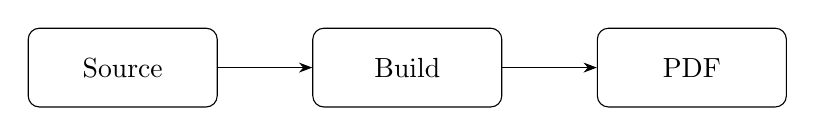
\begin{tikzpicture}[
  process node/.style={draw,rounded corners,minimum width=24mm,minimum height=10mm},
  node distance=12mm,>=Stealth]
  \node[process node] (source) {Source};
  \node[process node,right=of source] (build) {Build};
  \node[process node,right=of build] (pdf) {PDF};
  \draw[->] (source) -- (build);
  \draw[->] (build) -- (pdf);
\end{tikzpicture}
\end{center}
The arrows show a left-to-right transformation, not a feedback loop.

\section{A function plot}
\begin{center}
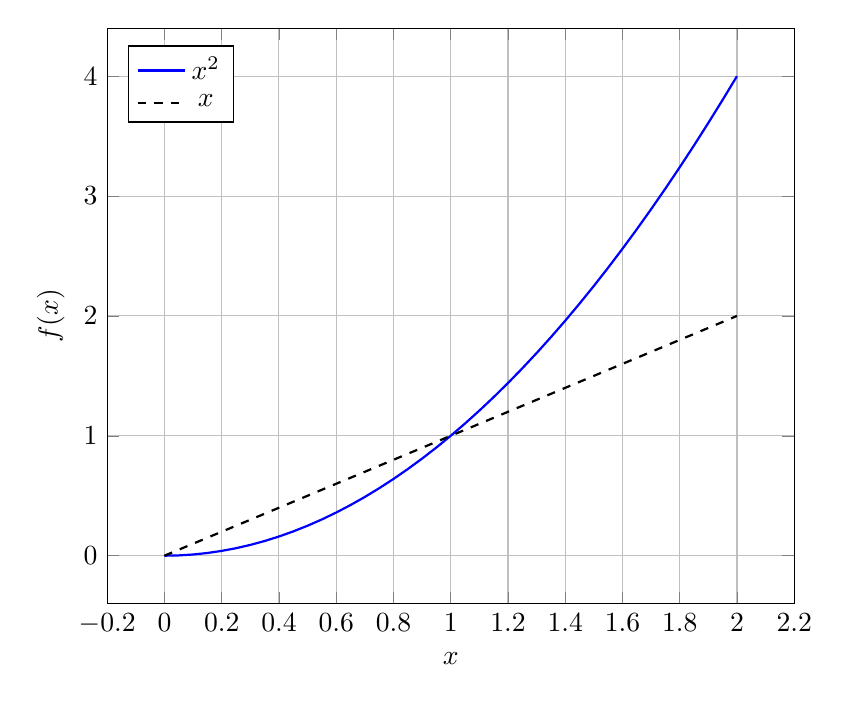
\begin{tikzpicture}
\begin{axis}[
  width=0.85\linewidth,
  xlabel={$x$},ylabel={$f(x)$},
  domain=0:2,samples=41,grid=major,
  legend pos=north west]
  \addplot[blue,thick,mark=none] {x^2};
  \addlegendentry{$x^2$}
  \addplot[black,dashed,thick] {x};
  \addlegendentry{$x$}
\end{axis}
\end{tikzpicture}
\end{center}
The curves intersect at \(x=0\) and \(x=1\). Line styles distinguish
the curves even without color.
\end{document}
